\appendixsection{Нагрузочное тестирование}

Для проведения нагрузочного тестирования было выбрано две конфигурации характеристик сервера БД.

Для начала продемонстрированы результаты выполнения с параметрами: CPU = 16, Memory = 32 GB, Hard Disk = 100 GB.

На рисунке~\ref{fig:b1} представлены результаты тестирования с параметрами «pgbench -i -s 10 database\_name», где флаг -s 100 указывает на размер масштабируемости данных, где 10 означает, что будет создано в 10 раз больше строк, чем количество таблиц.

\begin{figure}
    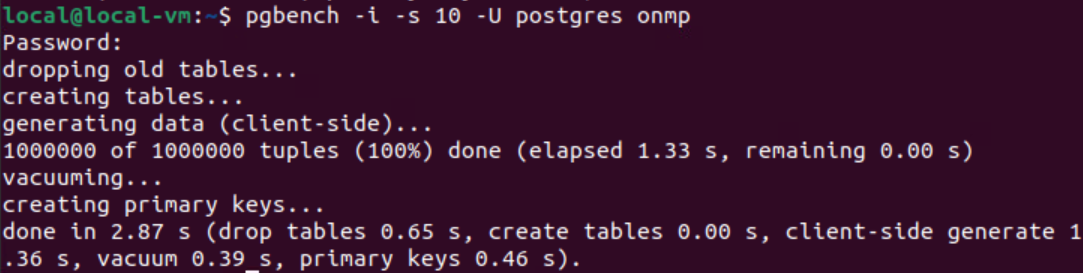
\includegraphics[width=16.5cm]{inc/test1_1}
    \caption{Тестирование с размером масштабируемости данных 10}
    \label{fig:b1}
\end{figure}

На рисунке~\ref{fig:b2} представлены результаты тестирования с параметрами «pgbench -i -s 100 database\_name».

\begin{figure}
    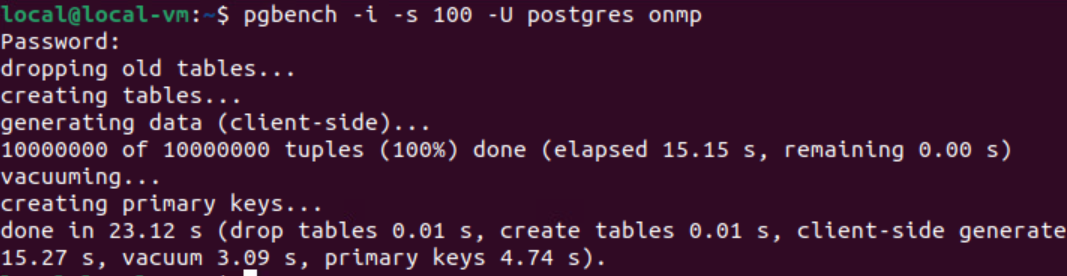
\includegraphics[width=16.5cm]{inc/test1_2}
    \caption{Тестирование с размером масштабируемости данных 100}
    \label{fig:b2}
\end{figure}

На рисунке~\ref{fig:b3} представлены результаты тестирования с параметрами «pgbench -i -s 1000 database\_name».

\begin{figure}
    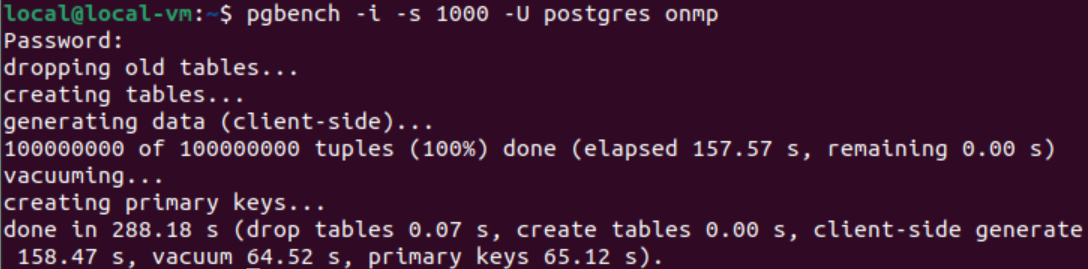
\includegraphics[width=16.5cm]{inc/test1_3}
    \caption{Тестирование с размером масштабируемости данных 1000}
    \label{fig:b3}
\end{figure}

На рисунке~\ref{fig:b4} представлены результаты тестирования с параметрами «pgbench -c 10 -j 10 -t 1000 database\_name», где флаг -c 10 указывает на количество параллельных клиентов, -j 10 указывает на количество параллельных потоков, а -t 1000 указывает на общее количество транзакций для выполнения.

\begin{figure}
    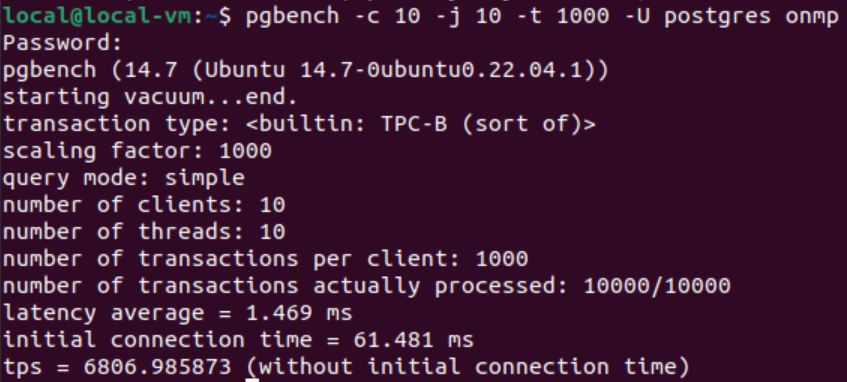
\includegraphics[width=16.5cm]{inc/test1_4}
    \caption{Тестирование с параметрами -c 10 -j 10 -t 1000}
    \label{fig:b4}
\end{figure}

На рисунке~\ref{fig:b5} представлены результаты тестирования с параметрами «pgbench -c 10 -j 10 -t 10000 database\_name».

\begin{figure}
    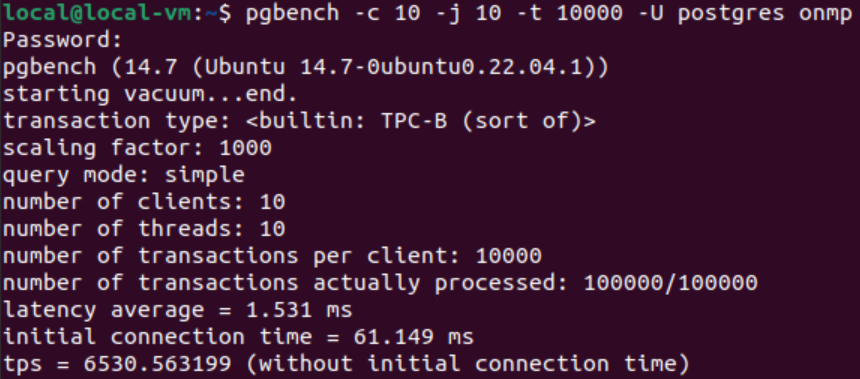
\includegraphics[width=16.5cm]{inc/test1_5}
    \caption{Тестирование с параметрами -c 10 -j 10 -t 10000}
    \label{fig:b5}
\end{figure}

На рисунке~\ref{fig:b6} представлены результаты тестирования с параметрами «pgbench -c 50 -j 50 -t 1000 database\_name».

\begin{figure}
    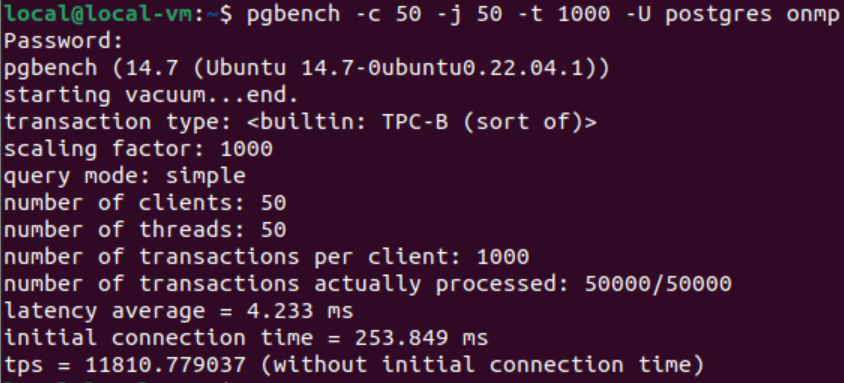
\includegraphics[width=16.5cm]{inc/test1_6}
    \caption{Тестирование с параметрами -c 50 -j 50 -t 1000}
    \label{fig:b6}
\end{figure}

На рисунке~\ref{fig:b7} представлены результаты тестирования с параметрами «pgbench -c 50 -j 50 -t 10000 database\_name».

\begin{figure}
    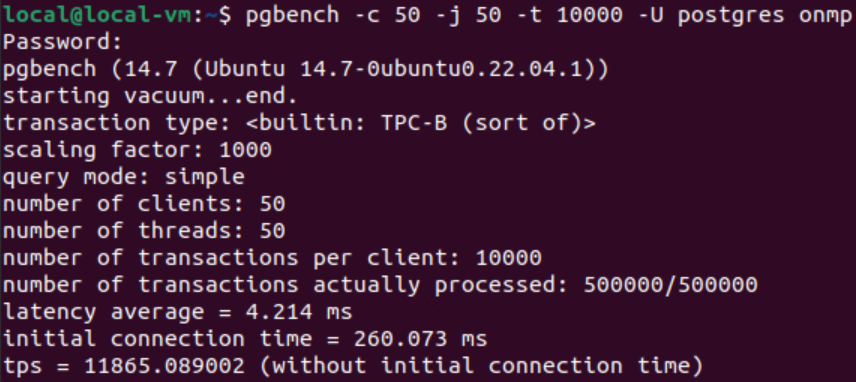
\includegraphics[width=16.5cm]{inc/test1_7}
    \caption{Тестирование с параметрами -c 50 -j 50 -t 10000}
    \label{fig:b7}
\end{figure}

На рисунке~\ref{fig:b8} представлены результаты тестирования с параметрами «pgbench -c 80 -j 80 -t 100000 database\_name».

\begin{figure}
    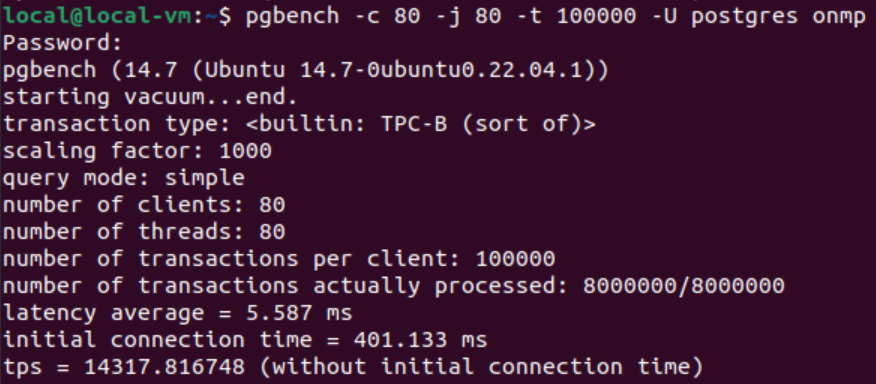
\includegraphics[width=16.5cm]{inc/test1_8}
    \caption{Тестирование с параметрами -c 80 -j 80 -t 100000}
    \label{fig:b8}
\end{figure}

Теперь изменим конфигурацию параметров системы: CPU = 32, Memory = 64 GB, Hard Disk = 200 GB.

На рисунке~\ref{fig:b9} представлены результаты тестирования с параметрами «pgbench -i -s 10 database\_name», где флаг -s 100 указывает на размер масштабируемости данных, где 10 означает, что будет создано в 10 раз больше строк, чем количество таблиц.

\begin{figure}
    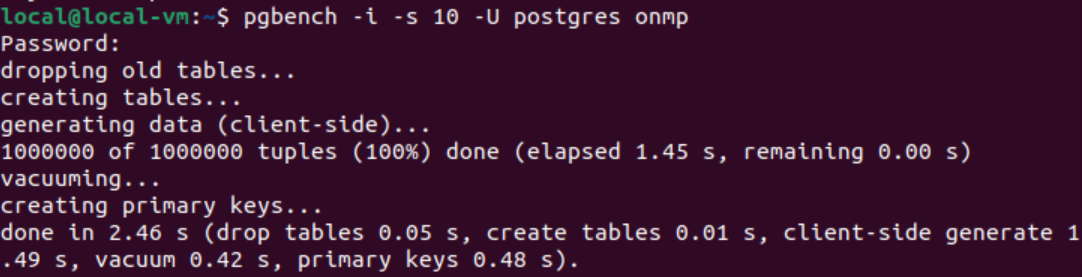
\includegraphics[width=16.5cm]{inc/test2_1}
    \caption{Тестирование с размером масштабируемости данных 10}
    \label{fig:b9}
\end{figure}

На рисунке~\ref{fig:b10} представлены результаты тестирования с параметрами «pgbench -i -s 100 database\_name».

\begin{figure}
    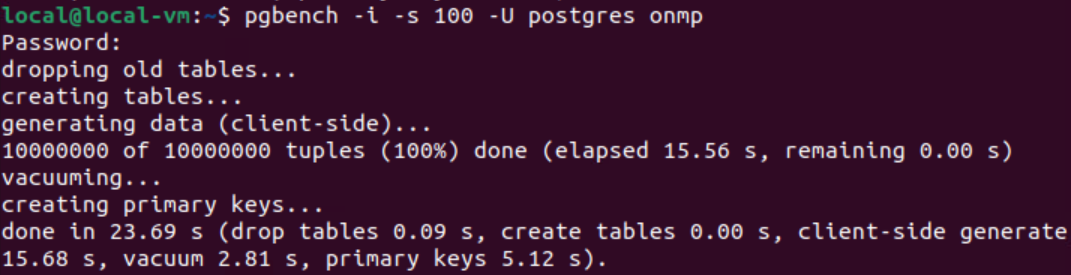
\includegraphics[width=16.5cm]{inc/test2_2}
    \caption{Тестирование с размером масштабируемости данных 100}
    \label{fig:b10}
\end{figure}

На рисунке~\ref{fig:b11} представлены результаты тестирования с параметрами «pgbench -i -s 1000 database\_name».

\begin{figure}
    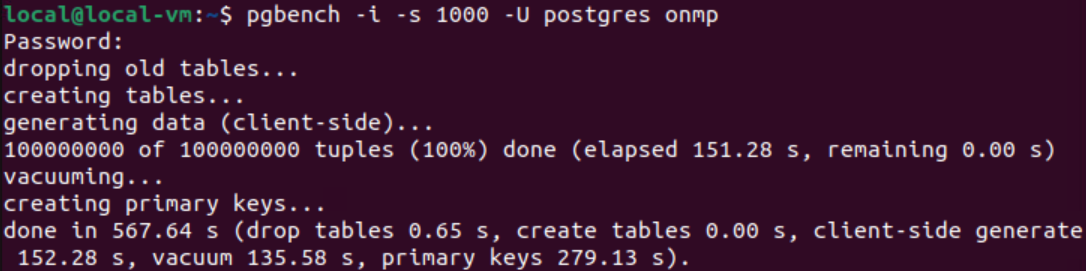
\includegraphics[width=16.5cm]{inc/test2_3}
    \caption{Тестирование с размером масштабируемости данных 1000}
    \label{fig:b11}
\end{figure}

На рисунке~\ref{fig:b12} представлены результаты тестирования с параметрами «pgbench -c 10 -j 10 -t 1000 database\_name», где флаг -c 10 указывает на количество параллельных клиентов, -j 10 указывает на количество параллельных потоков, а -t 1000 указывает на общее количество транзакций для выполнения.

\begin{figure}
    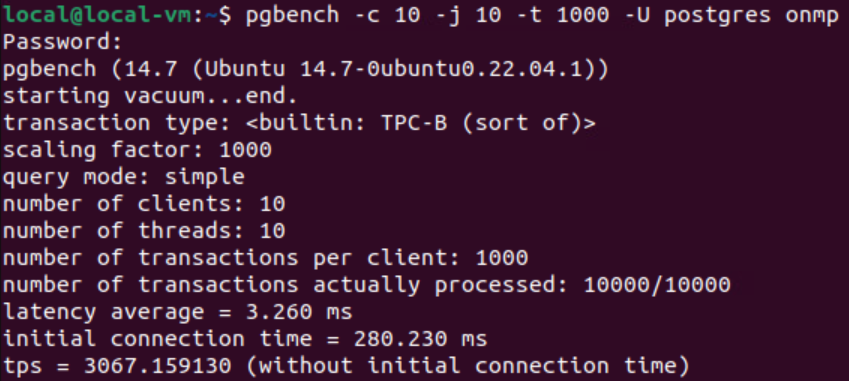
\includegraphics[width=16.5cm]{inc/test2_4}
    \caption{Тестирование с параметрами -c 10 -j 10 -t 1000}
    \label{fig:b12}
\end{figure}

На рисунке~\ref{fig:b13} представлены результаты тестирования с параметрами «pgbench -c 10 -j 10 -t 10000 database\_name».

\begin{figure}
    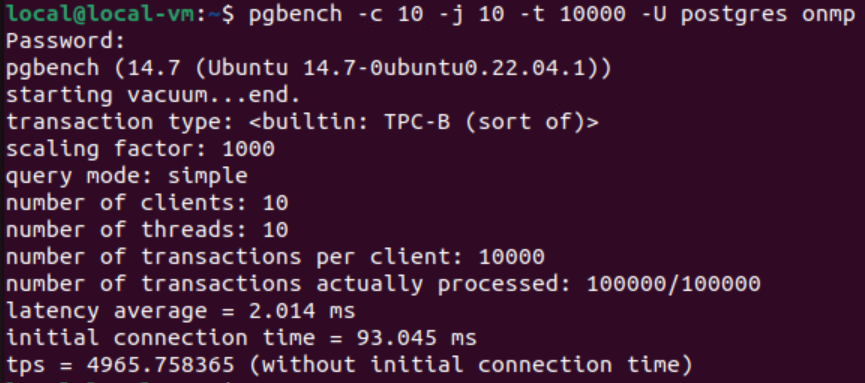
\includegraphics[width=16.5cm]{inc/test2_5}
    \caption{Тестирование с параметрами -c 10 -j 10 -t 10000}
    \label{fig:b13}
\end{figure}

На рисунке~\ref{fig:b14} представлены результаты тестирования с параметрами «pgbench -c 50 -j 50 -t 1000 database\_name».

\begin{figure}
    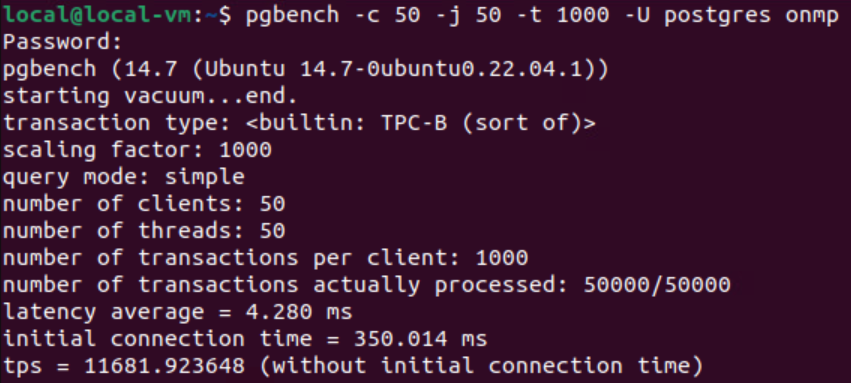
\includegraphics[width=16.5cm]{inc/test2_6}
    \caption{Тестирование с параметрами -c 50 -j 50 -t 1000}
    \label{fig:b14}
\end{figure}

На рисунке~\ref{fig:b15} представлены результаты тестирования с параметрами «pgbench -c 50 -j 50 -t 10000 database\_name».

\begin{figure}
    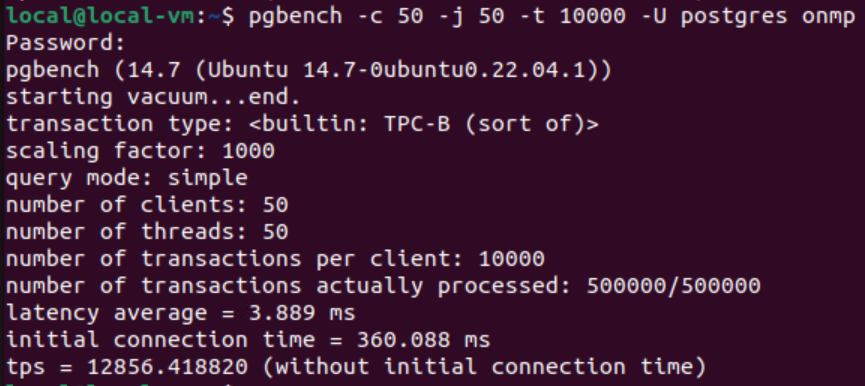
\includegraphics[width=16.5cm]{inc/test2_7}
    \caption{Тестирование с параметрами -c 50 -j 50 -t 10000}
    \label{fig:b15}
\end{figure}

На рисунке~\ref{fig:b16} представлены результаты тестирования с параметрами «pgbench -c 80 -j 80 -t 10000 database\_name».

\begin{figure}
    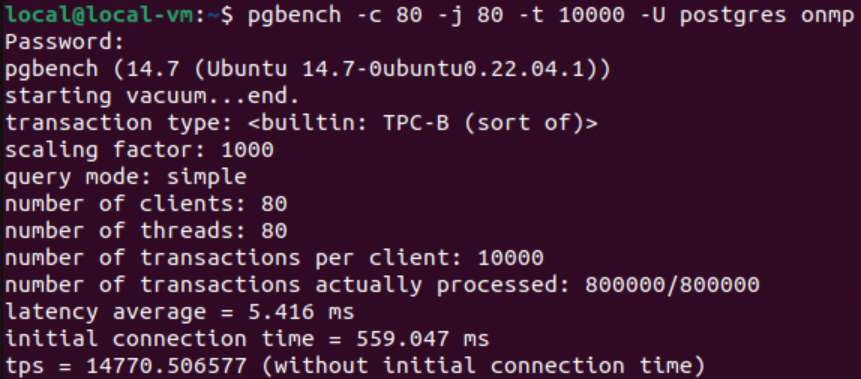
\includegraphics[width=16.5cm]{inc/test2_8}
    \caption{Тестирование с параметрами -c 80 -j 80 -t 10000}
    \label{fig:b16}
\end{figure}

На рисунке~\ref{fig:b17} представлены результаты тестирования с параметрами «pgbench -c 80 -j 80 -t 100000 database\_name».

\begin{figure}
    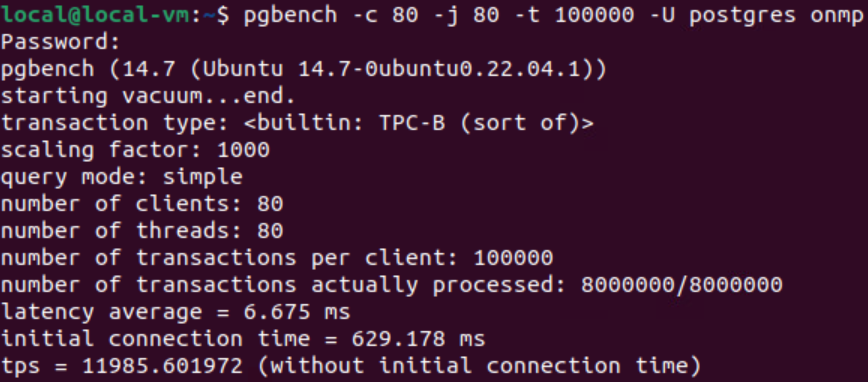
\includegraphics[width=16.5cm]{inc/test2_9}
    \caption{Тестирование с параметрами -c 80 -j 80 -t 100000}
    \label{fig:b17}
\end{figure}
